% Gemini theme
% See: https://rev.cs.uchicago.edu/k4rtik/gemini-uccs
% A fork of https://github.com/anishathalye/gemini

\documentclass[final]{beamer}

% ====================
% Packages
% ====================
\usepackage{amsfonts}
\usepackage[T1]{fontenc}
\usepackage{lmodern}
\usepackage[size=custom,width=120,height=72,scale=1.0]{beamerposter}
\geometry{paperwidth=42in,paperheight=32.5in}
\usetheme{gemini}
\usecolortheme{ucf}
\usepackage{graphicx}
\usepackage{booktabs}
\usepackage{tikz}
\usepackage{pgfplots}
\pgfplotsset{compat=1.17}

% ====================
% Lengths
% ====================

% If you have N columns, choose \sepwidth and \colwidth such that
% (N+1)*\sepwidth + N*\colwidth = \paperwidth
\newlength{\sepwidth}
\newlength{\colwidth}
\setlength{\sepwidth}{0.025\paperwidth}
\setlength{\colwidth}{0.3\paperwidth}

\newcommand{\separatorcolumn}{\begin{column}{\sepwidth}\end{column}}

% ====================
% Title
% ====================

\title{Impact of Travel and Schedule Density on NBA Performance}

\author{Aamogh B. Sawant \inst{1} \and Nathan Wright \inst{1}}

\institute[shortinst]{\inst{1} \textit{University of Central Florida, Orlando, FL} }

% ====================
% Footer (optional)
% ====================

\footercontent{
  \href{https://aamogh.vercel.app/}{aamogh.vercel.app} \hfill
  UCF Student Seminar, Orlando\hfill
  \href{mailto:aa031715@ucf.edu}{aa031715@ucf.edu}}
% (can be left out to remove footer)

% ====================
% Logo (optional)
% ====================

% use this to include logos on the left and/or right side of the header:
% \logoright{\includegraphics[height=7cm]{logo1.pdf}}
% \logoleft{\includegraphics[height=7cm]{logo2.pdf}}

% ====================
% Body
% ====================

\begin{document}
\addtobeamertemplate{headline}{}
{
    \begin{tikzpicture}[remember picture,overlay]
      \node [anchor=north west, inner sep=3cm] at ([xshift=0.0cm,yshift=3cm]current page.north west)
      {
\includegraphics[height=8.5cm]{logos/ucf_logo2.png}}; % also try shield-white.eps
      \node [anchor=north east, inner sep=3cm] at ([xshift=0.0cm,yshift=3cm]current page.north east)
      {\includegraphics[height=8.5cm]{logos/image.jpg}};
    \end{tikzpicture}
}

\begin{frame}[t]
\begin{columns}[t]
\separatorcolumn

\begin{column}{\colwidth}

  \begin{block}{Abstract}

  
Professional athletes operate under demanding schedules that require frequent travel, often across multiple time zones, which can have measurable effects on performance and overall well-being. In the National Basketball Association (NBA), factors such as travel distance, time zone shifts, and schedule density—particularly back-to-back games—are critical variables that influence player efficiency and team success.

This study employs a data-driven approach to quantify the impact of travel and scheduling constraints on key performance metrics, including shooting efficiency, defensive effectiveness, and turnover rates. Leveraging historical game data, we utilize both statistical and machine learning methodologies to identify trends and assess the extent to which travel-related fatigue affects player output. Our findings provide actionable insights for optimizing workload management, enhancing performance, and mitigating injury risks.



  \end{block}

\begin{block}{Methodology}

To rigorously analyze the impact of travel on NBA team performance, we employed a multi-faceted methodology that integrates data preprocessing, geospatial computation, statistical modeling, and advanced data visualization. Our approach ensures a robust and comprehensive examination of how travel-related fatigue influences key performance indicators across teams.

\textbf{Team Mapping and Data Standardization}: A crucial preprocessing step involved standardizing team identifiers to ensure consistency across datasets. Since raw NBA data often contains team abbreviations rather than full city names, we implemented a dictionary-based mapping strategy to enhance interpretability and facilitate dataset merging.

\textbf{Mapping Team Identifiers}:
\begin{itemize}
  \item A structured dictionary (team\_mapping) was created to associate NBA team abbreviations (e.g., ATL for Atlanta) with their full names.
  \item The mapping was applied via the .map() function in pandas to ensure uniformity.
\end{itemize}

\textbf{Integration with Game Data}:
\begin{itemize}
  \item The transformed dataset was merged with game performance statistics and travel data to establish a structured analytical framework.
  \item The standardized data was exported as a CSV file for downstream processing, ensuring consistency in feature engineering and model training.
\end{itemize}

This preprocessing step was essential for reducing inconsistencies and enabling a seamless analytical workflow.

\textbf{Derivation of Performance Metrics}: To quantify the impact of travel on player and team efficiency, we computed key performance metrics that capture offensive and defensive effectiveness. These metrics were derived using a combination of game statistics and normalization techniques to mitigate the influence of outlier performances.

\begin{itemize}
  \item \textbf{Offensive Rating (OffRtg)}: A measure of a team's scoring efficiency, calculated per 100 field goal attempts to normalize differences in pace across games. 
  $$ \text{OffRtg} = \left( \frac{\text{Team Points}}{\text{Field Goals Attempted}} \right) \times 100 $$

  \item \textbf{Defensive Rating (DefRtg)}: An analogous metric quantifying defensive efficiency, based on points allowed per 100 opponent field goal attempts. 
  $$ \text{DefRtg} = \left( \frac{\text{Opponent Points}}{\text{Opponent Field Goals Attempted}} \right) \times 100 $$

  \item \textbf{Offensive-to-Defensive Rating Ratio (OffDef Ratio)}: A composite metric assessing overall team efficiency by evaluating the balance between offensive and defensive effectiveness. 
  $$ \text{OffDef Ratio} = \frac{\text{OffRtg}}{\text{DefRtg}} $$
\end{itemize}



\end{block}



\end{column}

\separatorcolumn

\begin{column}{\colwidth}

  \begin{block}{Model}

    The analysis explored the impact of travel distance on NBA team performance using \textbf{linear regression models}, where the \textbf{Offensive-to-Defensive Rating Ratio (OffDef Ratio)} was the dependent variable, representing the efficiency balance between offense and defense, and \textbf{travel distance} (flight time in minutes) was the independent variable (predictor). 

To fit the models, the \textbf{Ordinary Least Squares (OLS)} regression method was used, which was implemented by the author, minimizing the difference between observed and predicted values. The regression equation was represented as:

\[
Y = \beta_0 + \beta_1 X + \epsilon
\]

Where:
\begin{itemize}
    \item \(Y\) is the OffDef Ratio,
    \item \(X\) is the travel distance,
    \item \(\beta_0\) is the intercept,
    \item \(\beta_1\) is the slope coefficient (showing how much \(Y\) changes for a unit change in \(X\)),
    \item \(\epsilon\) is the error term.
\end{itemize}

Regression analyses were conducted for each NBA team individually to identify team-specific trends, with a combined regression analysis across all teams revealing league-wide patterns. The \textbf{R-squared} and \textbf{p-values} were assessed to evaluate the strength and significance of the relationships between travel distance and performance.


The statistical models' reliability was validated using \textbf{R-squared values} to assess model fit and \textbf{p-values} to confirm the statistical significance of travel distance as a predictor of team performance. This comprehensive analysis revealed how travel influenced NBA team performance during the 2018 season, both on an individual team level and across the league.

  \end{block}

\begin{block}{Visualization}

    \begin{figure}[h!]
        \centering
        \begin{minipage}{0.8\textwidth} % Increase this to make the image larger
            \centering
            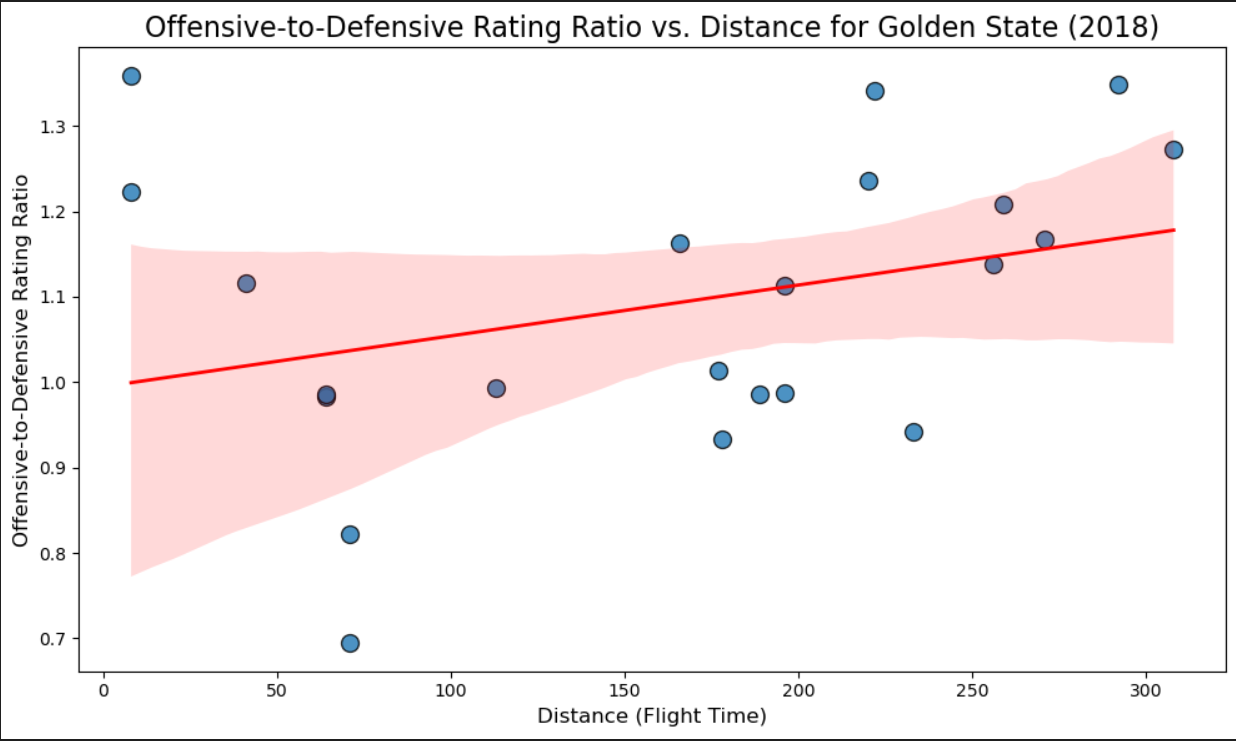
\includegraphics[width=\textwidth]{GoldenS.png} % First image
            \label{fig:first_image}
        \end{minipage} \hfill
        \begin{minipage}{0.8\textwidth} % Increase this to make the image larger
            \centering
            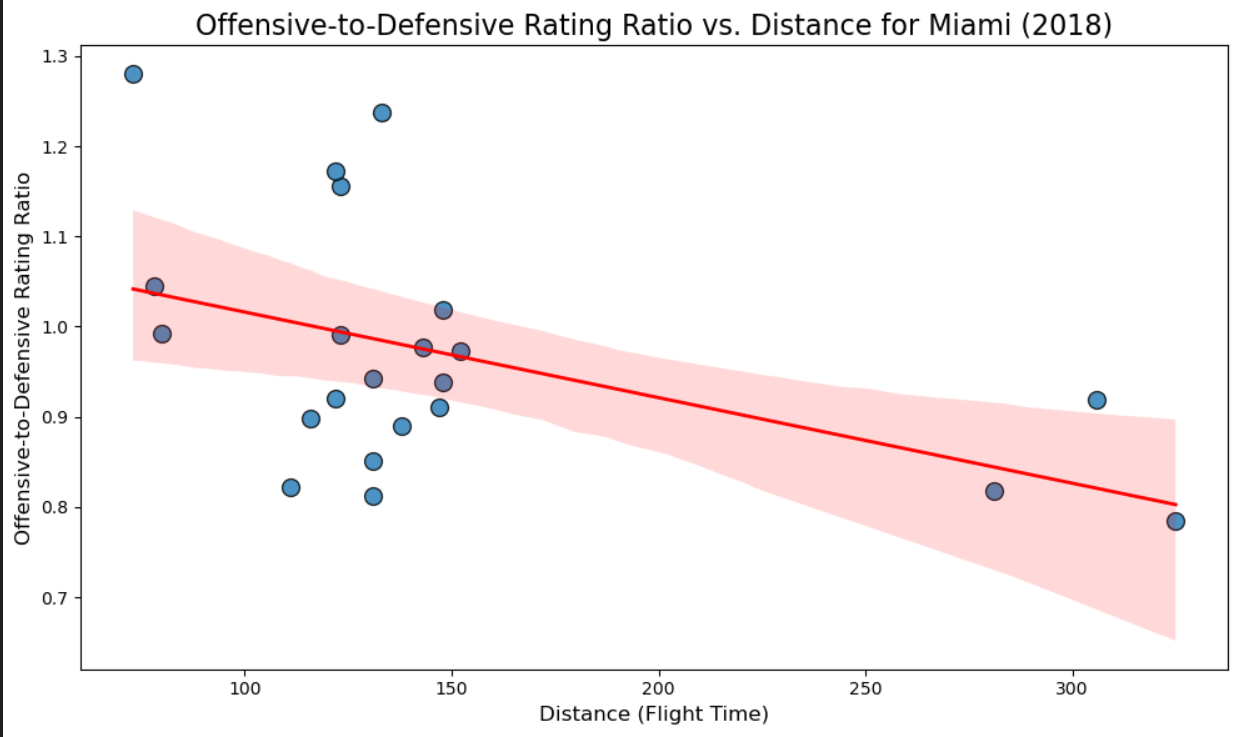
\includegraphics[width=\textwidth]{MiamiH.png} % Second image
            \label{fig:second_image}
        \end{minipage}
    \end{figure}

\end{block}




\end{column}

\separatorcolumn

\begin{column}{\colwidth}

  \begin{block}{Results}

    The statistical models were validated through iterative tests using R-squared values and p-values to assess the impact of travel distance on NBA team performance during the 2018 season.

At the league level, correlations between travel distance and performance (measured by the Offensive-to-Defensive Rating Ratio) varied:

\begin{itemize}
    \item \textbf{Positive correlations} were found for teams like the \textbf{LA Clippers (0.4843)}, \textbf{Golden State Warriors (0.3203)}, and \textbf{Toronto Raptors (0.4780)}, suggesting better performance with increased travel. This could be due to efficient travel arrangements and strong roster depth.
    \item \textbf{Negative correlations} appeared in teams like the \textbf{Miami Heat (-0.4675)}, \textbf{Portland Trail Blazers (-0.3751)}, and \textbf{Houston Rockets (-0.2603)}, indicating that longer travel hindered performance, likely due to fatigue or recovery issues.
    \item \textbf{Marginal correlations} were seen in teams like the \textbf{Chicago Bulls (0.0204)} and \textbf{Denver Nuggets (-0.0510)}, where travel had minimal impact on performance.
\end{itemize}

The variation across teams shows that travel affects performance differently, influenced by factors such as travel schedules, recovery strategies, and mental resilience.

  \end{block}

  \begin{block}{Future Directions}

    Future research could examine the effects of Ramadan fasting on players like Kyrie Irving, Jaylen Brown, Omer Yurtseven, Gorgui Dieng, and Enes Kanter Freedom, focusing on how fasting impacts shooting efficiency, stamina, and overall performance during road games. Integrating advanced tracking technologies and player analytics—such as real-time data on fatigue, heart rate, and energy expenditure—with traditional performance metrics could provide insights to optimize player performance, reduce fatigue, and minimize injury risks.


  \end{block}
  \begin{block}{Conclusion}

    This study explains the complex relationship between travel distances and the performance
of NBA teams, showing that the impact is substantially different across the teams—for
example, teams like Miami and Portland show a strong negative correlation, meaning long
travel distances hurt their performance. In contrast, teams such as the LA Clippers and
Golden State either thrive or are unaffected by greater travel distances. 


These findings bring
into the limelight the importance of developing team-specific strategies to mitigate travel’s
negative impact, which includes optimized travel schedules, recovery protocols, and how to
foster team chemistry during road trips. Future research should include individual player performance data and psychological factors via real-time tracking to better understand how
traveling affects each player’s efficiency in more detail and shape sports analytics for better
team management.

  \end{block}

  \begin{block}{References}

    \nocite{*}
    \footnotesize{\bibliographystyle{plain}\bibliography{poster}}

  \end{block}

\end{column}

\separatorcolumn
\end{columns}
\end{frame}

\end{document}
